\documentclass{article}
\usepackage[utf8]{inputenc}
\usepackage{graphicx}
\usepackage{todonotes}
\usepackage{url}
\usepackage[left=2.3cm,right=2.8cm, top = 2.2cm, bottom = 3cm]{geometry}


\title{Remarks on O'Driscoll et al, Clinical Infectious Diseases (2021)}
\author{J. Bracher, E. Brockhaus}
\date{August 2021}

\begin{document}

\maketitle

% \begin{abstract}
% O'Driscoll et al study the performance of various methods to estimate the basic reproductive number $R_0$ on simulated data. They conclude ``\textit{[...] that most methods considered here frequently overestimate $R_0$ in the early stages of epidemic growth on simulated data, the magnitude of which decreases when fitted to an increasing number of time points. This trend of decreasing bias over time can easily lead to incorrect conclusions about the course of the epidemic or the need for control efforts.''} We repeat their simulation study varying certain aspects and parameters. Our results suggest that the observed biases can be considerably reduced when aligning the chosen simulation approach and assumptions of the estimation methods more closely. In particular, it appears that the correct specification of the standard deviation of the generation time is crucial for the unbiasedness of estimates.
% \end{abstract}


\section{Background}

O'Driscoll et al study the performance of various methods to estimate the basic reproductive number $R_0$ on simulated data. They conclude ``\textit{[...] that most methods considered here frequently overestimate $R_0$ in the early stages of epidemic growth on simulated data, the magnitude of which decreases when fitted to an increasing number of time points. This trend of decreasing bias over time can easily lead to incorrect conclusions about the course of the epidemic or the need for control efforts.''} O'Driscoll et al (2020) follow high standards of reproducibility, enabling replication of their simulation experiments. We repeat their simulation study varying certain aspects and parameters. Our results suggest that the observed biases can be considerably reduced when aligning the chosen simulation approach and assumptions of the estimation methods more closely. In particular, it appears that the coherent specification of the standard deviation of the generation time is crucial for the unbiasedness of estimates.

%O'Driscoll et al (2020) compare seven different methods to estimate the basic reproductive number $R_0$ both on simulated and real-world data. In their simulation study they find that almost all methods frequently overestimate the true reproductive number when provided with short time series of case counts. This bias is found to diminish as more data become available. O'Driscoll et al (2020) follow high standards of reproducibility, enabling replication and variations of their simulation experiments. In this note we present some adaptions of their original analyses, which considerably reduce the observed biases.

\section{Simulation setting}

The employed simulation setting is described in Section S1 of the Supplementary Material of O'Driscoll et al. The authors employ a deterministic SEIR model with mean incubation time and infectious periods of 14 and 6 days, respectively. In the main analysis presented in the paper, daily incidences are obtained by rounding the values of the ODE curves to the nearest integer (results with Poisson or negative binomial noise are presented in the supplement). An underreporting factor of 0.2 is assumed and data are aggregated to a weekly resolution. All seven estimation methods are then applied to the weekly aggregated simulated data, varying the length of the available time series (6, 9, 12, and 15 weeks).

\section{Re-analysis using EpiEstim}

In the following we describe three variations of the simulation study performed by O'Driscoll et al. These aim to align the simulation setting and the assumptions of the EpiEstim method (Cori et al 2013) more closely. We only report results for this widely used approach.

\subsection{General simplifications/modifications of the simulation setting}

We adapt the simulation setting in a few ways which facilitate our analysis but are not expected to change overall results:
\begin{itemize}
\item To simplify the analysis we fix the total population number to $10^6$ rather than drawing it randomly.
\item As we also work with a stochastic SEIR model we only include values of $R_0$ of at least 2 as otherwise we run into issues with stochastic extinction.
\item For the same reason we increase the initial number of infected and sample it from a Unif(3, 8) rather than a Unif(1, 3) distribution.
\item We add fifty consecutive zeros at the beginning of the examined time series before feeding them into \texttt{EpiEstim::estimate\_R}. The \texttt{t\_start} argument in the call to \texttt{make\_config} is set to the second time point with strictly positive incidence in the respective time series. This is done because otherwise the \texttt{EpiEstim::estimate\_R} function throws the warning \texttt{"In check\_si\_distr(si\_distr, "warning") : si\_distr does not sum to 1."}
\item As we only consider the computationally fast EpiEstim method, we run 500 rather than 250 simulations.
\end{itemize}


\subsection{Adjusting the generation time distribution}

Drawing from Ferguson et al (2016), the authors assume a mean and standard deviation of the generation time of 20 and 7.4 days, respectively, in their application of the different estimation methods. While this assumption is thus in agreement with the biology of the Zika virus, it implies less variability of the generation time than the SEIR model used for simulation. This model implies that the mean and standard deviation of the incubation period are both 14 days, while the mean and standard deviation of the infectious period are both 6 days. The generation time then has a mean of $14 + 6 = 20$ days and a standard deviation of $\sqrt{14^2 + 6^2} = 15.23$. In a first step we therefore re-run all analyses using this standard deviation for the generation time.

As stated by Park et al (2020), ``a generation-interval distribution
that has a larger mean [...] or is less variable [...] gives
a higher estimate of $R_0$ for the same [growth rate].'' We thus expect the estimates to become lower when adjusting the generation time distribution to 15.25 days.



\subsection{Estimation based on daily data}

Motivated by their real-data example, O'Driscoll et al aggregate all simulated data to a weekly scale. The mean and standard deviation of the generation time on a weekly scale are obtained by dividing their counterparts on a daily scale by seven. While this seems intuitively reasonable, it is not obvious which impact this way of coarsening of the generation time distribution may have on the estimated reproductive numbers. We therefore remove this layer of complexity and omit the aggregation step from the simulation. The estimation is thus performed using data on a daily scale.


\subsection{Making the data-generating process fully stochastic}

Most of the considered methods assume that the epidemic process is inherently stochastic. Moreover, they operate in discrete time and treat cases as a truly discrete quantity. The data-generating process used by O'Driscoll et al, on the other hand, is deterministic (apart from observation noise added in some scenarios), operates in continuous time and treats cases as a continuous quantity. As we are most interested in the early phase of an epidemic, when incidence is low and stochastic fluctuations can matter, it is unclear whether this difference between simulation model and assumptions for estimation can have an impact on results. We therefore replace the deterministic SEIR model by a simple stochastic version in discrete time, similar to a time series SIR (TSIR) model (Bj{\o}rnstad 2002). Briefly summarizing the model, we simulate the transitions between the different compartments in discrete time via binomial sampling steps with appropriately chosen transition probabilities based on the respective parameters of the SEIR model.

\section{Results}

In our adapted simulation setting, the biases when using a standard deviation of 7.4 days for the generation time are slightly larger than in the manuscript, but qualitatively similar.

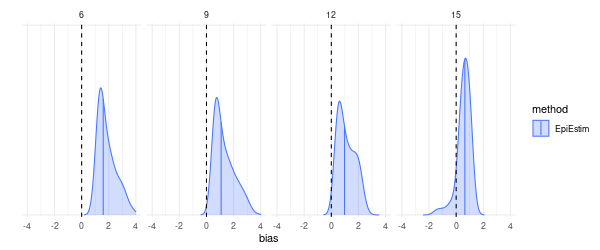
\includegraphics[scale=0.53]{figures/bias_7.png}

As expected, when we increase the standard deviation of the generation time we obtain lower estimates of $R_0$. Indeed, the majority of the bias is removed by this adjustment:

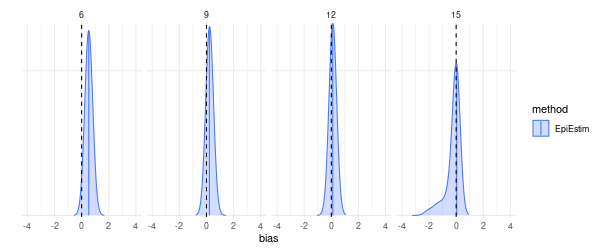
\includegraphics[scale=0.53]{figures/bias_15.png}

It further decreases when providing the model with daily rather than weekly data. Indeed, we observe that the sign of the bias changes when using 105 days of data.

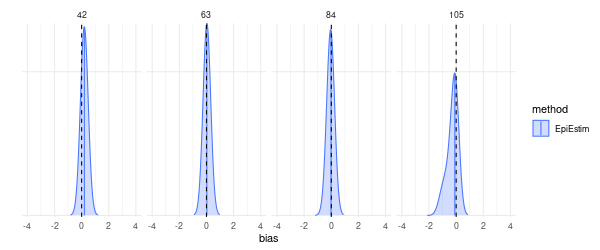
\includegraphics[scale=0.53]{figures/bias_15_daily.png}

When moving to the stochastic data simulation we obtain unbiased estimates for 42 weeks of data, while there is a slightly more pronounced downward bias in estimates for longer time series. For the shorter time series we now observe increased variability of the estimates, which is reasonable given that the generating model now involves stochasticity.

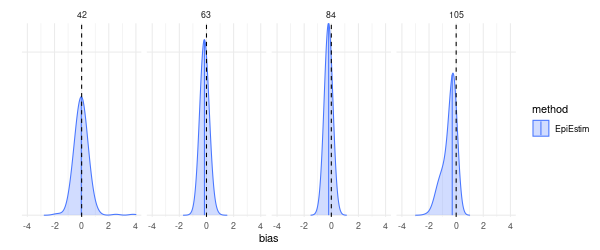
\includegraphics[scale=0.53]{figures/bias_15_daily_stoch.png}

From these results we infer that the EpiEstim method is unbiased if its assumptions are in agreement with the characteristics of the data-generating process and if a short time series is provided. If a longer time series is used, the estimates are biased downwards due to a reduction of the (effective) reproductive number following depletion of susceptibles. This interpretation is in line with the patterns seen in scatter plots of the individual estimates. Here, it can be seen that for large values of $R_0$ and time series of 15 weeks, there is a considerable downward bias in the estimated $R_0$. This bias is absent or less pronounced for smaller values of $R_0$ as in this case the susceptible pool is not or only slightly depleted after 15 weeks.

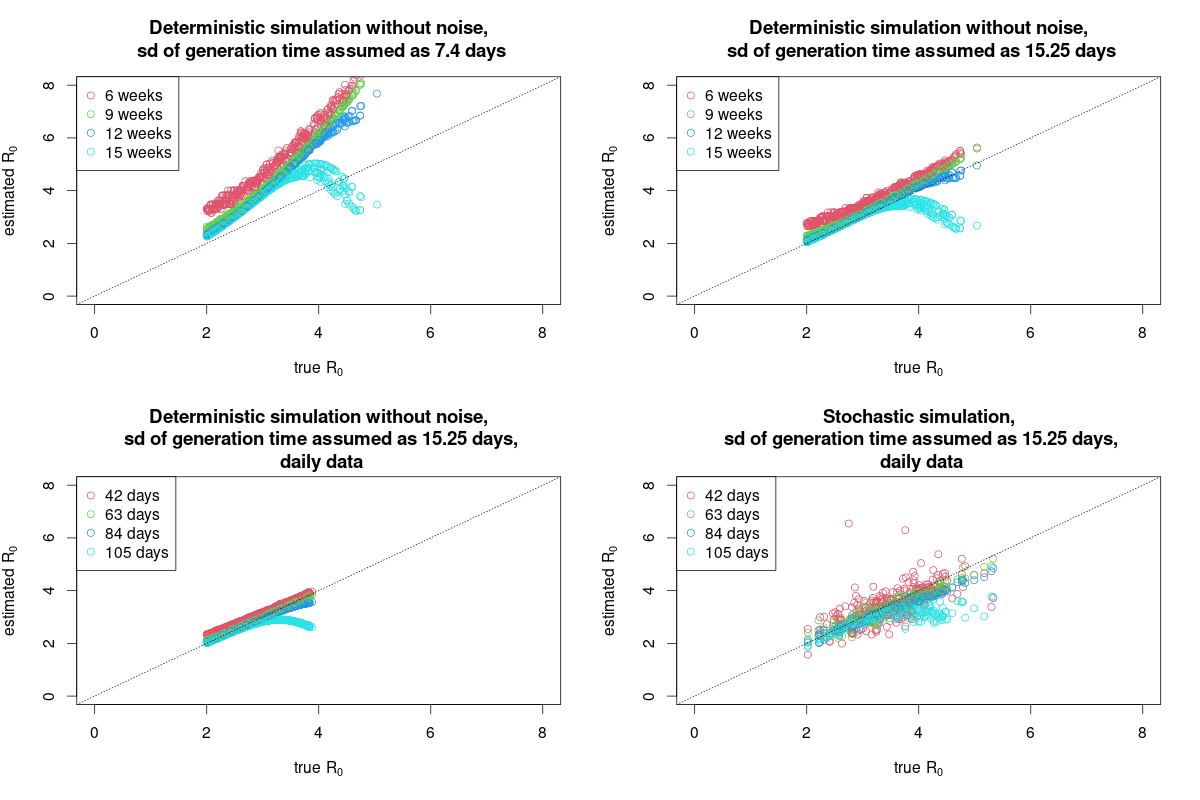
\includegraphics[scale=0.34]{figures/scatterplots.png}

\section*{Code}

Codes to generate all figures can be found in \url{https://github.com/ElisabethBrockhaus/R0-methods-comparison}.

\section*{References}

\begin{description}
\item O'Driscoll et al (2020): A Comparative Analysis of Statistical Methods to Estimate the Reproduction Number in Emerging Epidemics, With Implications for the Current Coronavirus Disease 2019 (COVID-19) Pandemic. Clinical Infectious Diseases 73(1):e215–23.
\item Cori et al (2013): A New Framework and Software to Estimate Time-Varying Reproduction Numbers During Epidemics. American Journal of Epidemiology 178(9):1505--1512.
\item Ferguson et al (2016): Countering the Zika epidemic
in Latin America. Science 353(6297), 353--354.
\item Park et al (2020): Reconciling early-outbreak estimates of the basic reproductive number and its uncertainty: framework and applications to the novel coronavirus (SARS-CoV-2) outbreak. Journal of the Royal Society Interface 17:20200144.
\item Bj{\o}rnstad et al (2002): Dynamics of Measles Epidemics: Estimating Scaling of Transmission Rates Using a Time Series SIR Model.  Ecological Monographs 72(2), 169--184.
\end{description}

\end{document}
